\chapter{Machine Learning Operations}

% TODO Tarvitseeko luku omaa pientä introa?
% Luvun scope
%This chapter introduces the basic concepts of ML in \autoref{sec:ml} and basic concepts of DevOps in \autoref{sec:devops}. Finally in \autoref{sec:mldevops} DevOps and ML are combined to form a new concept of MLOps.

%--------------------------------------------------------------------------------------------------------------------------------------------
\section{Machine Learning} % 2 pages
\label{sec:ml}

\subsection{Overview}

Writing programs and developing algorithms to complete specific tasks is a labor intensive task requiring professional programming expertise. A different approach is to develop generic algorithms that can change behavior by learning. The field studying these types of algorithms is called machine learning.

Machine learning is widely used in applications like search, drug design or ad placement and can be also known as data mining or predictive analytics \parencite{domingosFewUsefulThings2012}. Developing machine learning systems can be a difficult task. Unlike traditional software development, experiments with both code and data as inputs are central to machine learning development \parencite{zahariaAcceleratingMachineLearning2018} and reproducibility of the experiments is problematic. While plenty of research focuses on machine learning methods or even datasets and data quality, the biggest bottleneck is human cycles \parencite{domingosFewUsefulThings2012}. One important metric to pay attention to and optimize is the mean iteration cycle for machine learning developers.



%TODO more references
Machine learning can be practiced with two different goals in mind. First is explanatory modeling with the purpose of scientific theory building and testing and the second is predictive modeling mostly used outside of scientific research \parencite{shmueliExplainPredict2010a}. One practical difference is that unlike predictive modeling, explanatory modeling rarely uses holdout test sets or cross validation for evaluation \parencite{shmueliExplainPredict2010a}. Lack or presence of evaluation on a test set can be used as a heuristic to quickly determine whether a machine learning project is explanatory or predictive in nature. However, even explanatory modelling benefits from evaluating the predictive power \parencite{shmueliExplainPredict2010a}. Domingos \parencite*{domingosFewUsefulThings2012} in their paper assume all machine learning is predictive in nature and state the following: \begin{quote}
    The fundamental goal of machine learning is to generalize beyond the examples in the training set.
\end{quote}
It is important to keep in mind the end goals of a machine learning project, because common practices might not be applicable.

TODO Types of machine learning, get references

Unsupervised learning has the advantage of not requiring labeled data which is an advantage for problems where labels are uncommon \parencite{leBuildingHighlevelFeatures2012}. Unsupervised pretraining or feature learning on large datasets can yield to surprising results such as human facial recognition \parencite{leBuildingHighlevelFeatures2012}. Unsupervised machine learning techniques can be used as part of a learning pipeline as a preprocessing or postprocessing step even if the rest of the system uses supervised machine learning.

TODO ML model lifecycle, get references

\subsection{Machine learning algorithms}

TODO Model evaluation


\subsection{Hyperparameter optimization}

Parameters given as part of a configuration to the machine learning model are called hyperparameters \parencite{yangHyperparameterOptimizationMachine2020}. Hyperparameter selection is a difficult and automatic tuning of hyperparameters can help achieve state-of-the-art performance \parencite{maclaurinGradientbasedHyperparameterOptimization2015}. Hyperparameter optimization techniques include grid search, random search, gradient based optimization and Bayesian optimization and they have different benefits and limitations \parencite{yangHyperparameterOptimizationMachine2020}.

Neural Architecture optimization and Meta modeling are similar to hyperparameter optimization where model structure or modeling algorithm is treated as a tunable parameter \parencite{bakerAcceleratingNeuralArchitecture2017}. Traditional hyperparameter tuning methods such as Bayesian optimization are unfeasible for more than 10-20 hyperparameters \parencite{maclaurinGradientbasedHyperparameterOptimization2015}.

Performance prediction is an important step to reduce the amount of computation required for neural architecture search and hyperparameter optimization \parencite{bakerAcceleratingNeuralArchitecture2017}. TODO early stopping reference.



%--------------------------------------------------------------------------------------------------------------------------------------------
\section{DevOps} % 2 pages
\label{sec:devops}

\subsection{Overview}

%TODO 1. Intro to DevOps and definition mishra2020, waller2015

There is little consensus on the exact definition of DevOps \parencite{smedsDevOpsDefinitionPerceived2015}. Most commonly DevOps is said to have a focus on software quality, collaboration between development and operations, process speed and rapid feedback \parencite{mishraDevOpsSoftwareQuality2020,wallerIncludingPerformanceBenchmarks2015, pereraImproveSoftwareQuality2017}. DevOps can be viewed from different points of view such as culture, collaboration, automation, measurements and monitoring \parencite{mishraDevOpsSoftwareQuality2020, wallerIncludingPerformanceBenchmarks2015}. This section will describe measurement, monitoring and automation parts of DevOps in more detail.

% TODO 2. 


Continuous integration, continuous deployment and continuous monitoring are well known practices in DevOps \parencite{wallerIncludingPerformanceBenchmarks2015} describing the automatic nature of integrating, deploying and monitoring code changes. Performance profiling and monitoring are similar activities and the main difference is whether it's done during the development process or during operations respectively \parencite{wallerIncludingPerformanceBenchmarks2015}. DevOps bridges the gap between evaluating performance during the development process and during operations \parencite{brunnertPerformanceorientedDevOpsResearch2015}.

TODO Devops lifecycle steps

\begin{figure}[h]
    \centering
    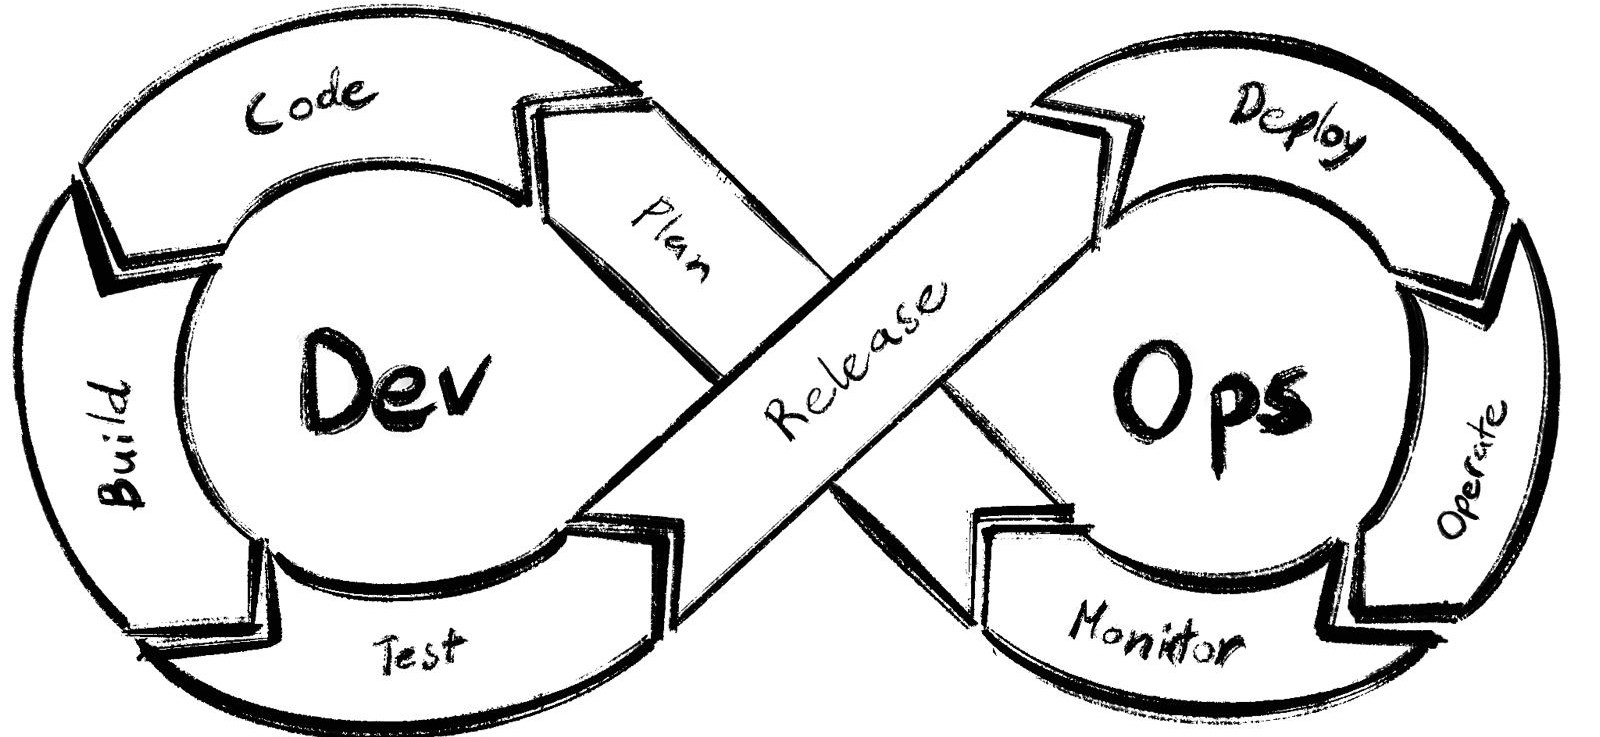
\includegraphics[width=0.75\textwidth]{devops.jpg}
    \caption{Example of a typical DevOps lifecycle}
    \label{fig:devops}
\end{figure}


TODO resource allocation/resource consumption, small memory software, benchmarking

\subsection{Measurement and monitoring}

Performance metrics are fundamental to all activities involving performance evaluation such as profiling or monitoring \parencite{brunnertPerformanceorientedDevOpsResearch2015}. Common metrics involve measuring the CPU, but other metrics such as memory usage, network traffic or I/O usage are not as well defined as a CPU metric \parencite{brunnertPerformanceorientedDevOpsResearch2015}.

\begin{itemize}
    \item Task Completion time
    \item Throughput
    \item Latency
    \item CPU usage
    \item GPU usage
    \item RAM usage
    \item VRAM usage
    \item I/O usage
    \item Network traffic
\end{itemize}

\subsection{Continuous optimization?}

Preprocessing

Training

Serving Latency

Resource demands might change depending on the inputs \parencite{brunnertPerformanceorientedDevOpsResearch2015} making it important to systematically measure performance not only based on code changes but also on configuration changes or even data changes.

%--------------------------------------------------------------------------------------------------------------------------------------------
\section{MLOps} % 4 pages
\label{sec:mldevops}

\subsection{Overview}

TODO \parencite{kreuzbergerMachineLearningOperations2022} data scientists doing manual work issue from conclusions, definition of MLOps, limit to technical stuff and tooling

%TODO rajaa devops teknisiin asioihin
Requirements for a machine learning system are different depending on the task. For example speech and object recognition might have no particular performance requirements during training but strict latency and computational resource restrictions when deployed to serve large amounts users \parencite{hintonDistillingKnowledgeNeural2015}. One of the key areas of MLOps is using machine learning in production systems in addition to data processing and machine learning model training.

Performance measuring software is not new, but ML brings additional challenges in the form of models and data which requires a modified approach \parencite{breckMLTestScore2017a}. It is also important to note, that not every data scientist or machine learning engineer working on machine learning systems has a software engineering background \parencite{finzerDataScienceEducation2013} and might lack the necessary knowledge to apply software engineering best practices to machine learning systems.

TODO MLOps lifecycle steps

\begin{figure}[h]
    \centering
    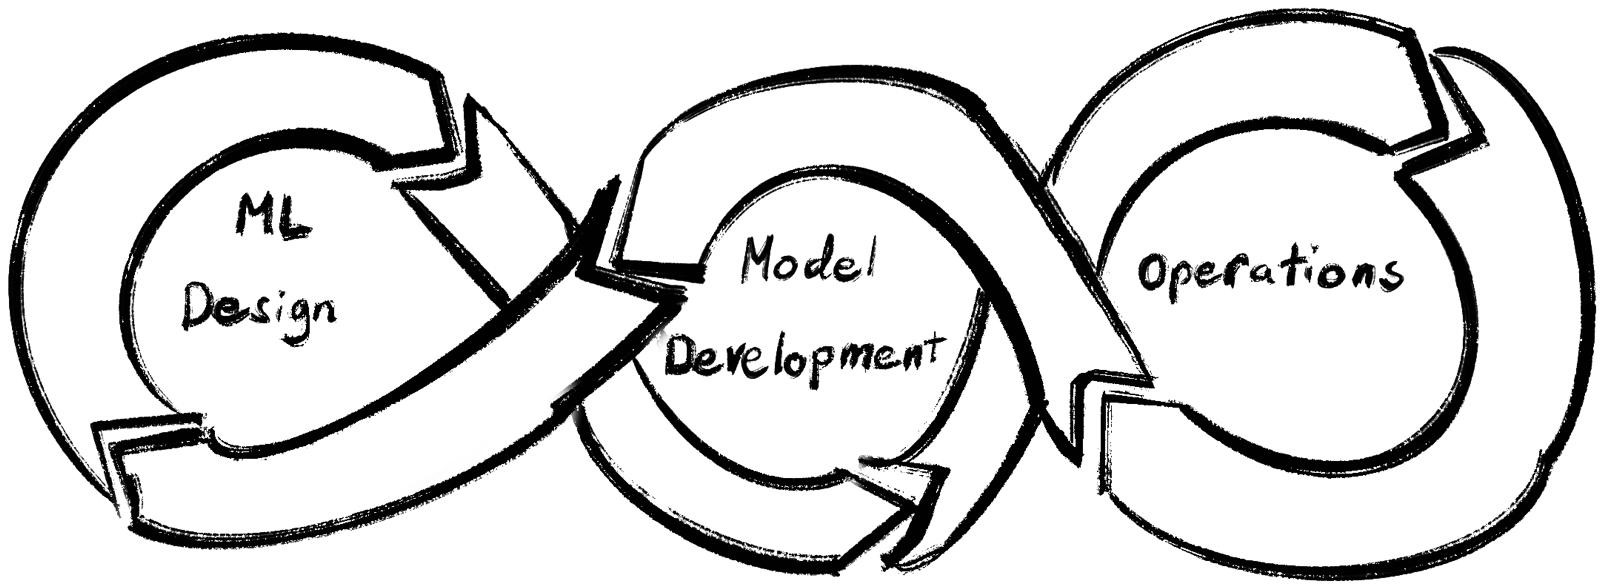
\includegraphics[width=0.75\textwidth]{mlops.jpg}
    \caption{Example of a typical MLOps lifecycle}
    \label{fig:mlops}
\end{figure}

TODO what DevOps brings to ML

TODO Continuous Training

\subsection{AutoML}

Machine learning systems in addition to machine learning performance metrics and system performance metrics will have their performance metrics tied to product or organization metrics such as user churn rate or click-through rate \parencite{shankarOperationalizingMachineLearning2022}. Choosing the right metrics to evaluate a machine learning system is important and the metrics will be different for different machine learning systems \parencite{shankarOperationalizingMachineLearning2022}.

Automated Machine Learning (AutoML) aims to minimize human intervention in completing data analytics tasks using machine learning algorithms \parencite{yangIoTDataAnalytics2022}.

\subsection{Performance prediction and early stopping}

